\documentclass[11pt,mathserif]{beamer} %You need this at the top to declare that you're using Beamer 

%----------------------------------------------------------------------------------------------------------------------------------------------%
%%%%%%%%% Before we start putting the presentation together, need to declare formating and packages %%%%

%%%%%%%%%%%%%%% Standard packages%%%%%%%%%%%%%%%
\usepackage{algorithm,algorithmic}  %2 packages for making nice looking algorithms
\usepackage{amsmath,mathtools} %Standard math commands (like vectors, symbols, etc.)
\usepackage{epsfig,epstopdf} %You need these if you have .eps vector graphics (recommend if possible)
%\usepackage{tikz} %Sometimes you may want to use Tikz to make figures (but its pretty complicated)
\usepackage{media9} %If you want to include movies (like in my earlier presentation) you'll need this package
%%% Below are packages commonly used for making figures
\usepackage{subfigure,MnSymbol,pdfpages}
\usepackage{graphicx,color,colortbl}
\usepackage{bm,amsfonts,graphics}

\usepackage{listings} %You won't need this unless youre displaying source code - I DONT RECOMMEND YOU DO THIS YET



%%%%%%%%%%%%%%% Commands for making the ACL slide format %%%%%%%%%%%%%%%%%
\setbeamercolor{block title}{bg=blue!55,fg=black}%bg=background, fg= foreground
\setbeamercolor{block body}{bg=blue!20,fg=black}%bg=background, fg= foreground
\renewcommand{\vec}[1]{\mathbf{#1}} %Changes the ``vec'' command for vectors to bold font rather than arrows overhead
\usepackage{amsmath}
\usepackage{mathtools}
\usepackage{tikz}
%\usepackage{movie15}
\usepackage{algorithm} % must read after hyperref
\usepackage{algorithmic}
\usepackage{subfigure,MnSymbol}
\usepackage{graphicx,color,colortbl}
%\usepackage[footnotesize,bf]{caption}
\usepackage{bm,amsfonts,graphics}
\usepackage{tikz,tkz-graph,tkz-arith,tkz-berge}
\usetikzlibrary{arrows,shapes,positioning}

\graphicspath{{./}{figures/}}
\usepackage{multicol}

\newtheorem{thm}{Theorem}
\newtheorem{lem}{Lemma}
\newtheorem{prop}{Proposition}
\newtheorem{rem}{Remark}

\newcommand{\jcols}[4]{
\begin{columns}[T]\begin{column}[T]{#3\textwidth} #1 \end{column}
\begin{column}[T]{#4\textwidth} #2 \end{column}
\end{columns}}

\newcommand{\jcolsb}[4]
{\begin{columns}[b]
\begin{column}{#3\textwidth} #1 \vspace{0pt}
\end{column}
\begin{column}{#4\textwidth} #2 \vspace{0pt}
\end{column}
\end{columns}}

\newcommand{\jcolsc}[4]
{\begin{columns}[c]
\begin{column}{#3\textwidth} #1 \vspace{0pt}
\end{column}
\begin{column}{#4\textwidth} #2 \vspace{0pt}
\end{column}
\end{columns}}
\mode<presentation>
{
	\usetheme{ACL}
        \setbeamercovered{transparent=0}
}

\makeatletter
\newdimen\labelwidthi
\newdimen\labelwidthii
\newdimen\labelwidthiii
\newdimen\labelwidthiv
\def\normal@labelsep{0.2em}
\labelsep\normal@labelsep
\settowidth{\labelwidthi}{iii}
\settowidth{\labelwidthii}{ii}
\settowidth{\labelwidthiii}{iii}
%\settowidth{\labelwidthiv}{i}
\setlength\leftmargini{0pt}
\setlength\leftmarginii{1.5ex}
\setlength\leftmarginiii{1.5ex}

\leftmargini\labelwidthi    \advance\leftmargini\labelsep
\leftmarginii\labelwidthii  \advance\leftmarginii\labelsep
\leftmarginii\labelwidthiii \advance\leftmarginiii\labelsep

%\leftmarginii\labelwidthiv  \advance\leftmarginiv\labelsep
%\def\setleftmargin#1#2{\settowidth{\@tempdima}{#2}\labelsep\normal@labelsep
%  \csname labelwidth#1\endcsname\@tempdima
%  \@tempdimb\@tempdima \advance\@tempdimb\labelsep
%  \csname leftmargin#1\endcsname\@tempdimb}
%\def\@listI{\leftmargin\leftmargini
%  \labelwidth\labelwidthi \labelsep\normal@labelsep
%  \topsep \z@ \partopsep\z@ \parsep\z@ \itemsep\z@
%  \listparindent 1em}
%\def\@listii{\leftmargin\leftmarginii
%  \labelwidth\labelwidthii \labelsep\normal@labelsep
%  \topsep\z@ \partopsep\z@ \parsep\z@ \itemsep\z@
%  \listparindent 1em}
%\def\@listiii{\leftmargin\leftmarginiii
%  \labelwidth\labelwidthiii \labelsep\normal@labelsep
%  \topsep\z@ \partopsep\z@ \parsep\z@ \itemsep\z@
%  \listparindent 1em}
%\def\@listiv{\leftmargin\leftmarginiv
%  \labelwidth\labelwidthiv \labelsep\normal@labelsep
%  \topsep\z@ \partopsep\z@ \parsep\z@ \itemsep\z@
%  \listparindent 1em}
%\let\@listi\@listI
%\@listi
\makeatother

\logo{

\includegraphics[height = 0.6cm,trim=0 50 0 0,clip]{AO-logo-high_color-top-MIT}

\includegraphics[height = 0.5cm,trim=0 0 0 0,clip]{ACL_logo}
}

\setbeamerfont{frametitle}{size=\large,series=\bfseries}
%\setbeamertemplate{frametitle}[default][center]
\setbeamerfont{title}{size=\large,series=\bfseries}
\setbeamerfont{framesubtitle}{series=\mdseries,size=\large}
\graphicspath{{./}{figures/}}
\usepackage[square, numbers, comma]{natbib}	% use Natbib for author-name
									% citations. In a presentation,
									% this is more legible than pure
									% numbers, like [21]. Google
									% "natbib" for more information.
									% Instead of "\cite{abc}", use
									% "\citep{abc}" or "\citet{abc}"
\bibliographystyle{plainnat}		% Natbib specific
%\bibpunct{(}{)}{,}{a}{}{,}			% Natbib specific

\definecolor{Maroon}{RGB}{112,0,0}
\definecolor{Crimson}{RGB}{200,0,0}
\definecolor{purple}{RGB}{112,0,112}

\newcommand{\bee}{\begin{enumerate}}
\newcommand{\eee}{\end{enumerate}}
\newcommand{\bi}{\begin{itemize}}
\newcommand{\bii}{\begin{itemize}\small}
\newcommand{\beee}{\begin{enumerate}\scriptsize}
\newcommand{\biii}{\begin{itemize}\footnotesize}
\newcommand{\ei}{\end{itemize}}
\newcommand{\jtem}{\vfill\item}
\newcommand{\bea}{\begin{eqnarray}}
\newcommand{\eea}{\end{eqnarray}}
\newcommand{\argmax}{\operatornamewithlimits{argmax}}
\newcommand{\njra}{\color{red} $\Rightarrow$~\color{black}}
\newcommand{\nred}[1]{{\tiny \color{red} XX #1 XX\color{black}}}
%\newcommand{\jframe}[1]{\begin{frame}\nred{#1}\end{frame}}
\newcommand{\jframe}[2]{\begin{frame}\frametitle{#1} #2 \end{frame}}
\newcommand{\jframeb}[2]{\begin{frame}[t]{#1} \begin{itemize} #2 \end{itemize} \end{frame}}
\newcommand{\jframet}[2]{\begin{frame}[t]\frametitle{#1} #2 \end{frame}}
\newcommand{\ji}[2]{\begin{itemize}\setlength{\itemsep}{#1mm}{#2}\end{itemize}}
\newcommand{\jen}[2]{\begin{enumerate}\setlength{\itemsep}{#1mm}{#2}\end{enumerate}}
\newcommand{\bc}{\begin{center}}
\newcommand{\ec}{\end{center}}
\newcommand{\todo}[1]{{\color{magenta} XX- #1 -XX}}
\newcommand{\XX}[1]{{\color{red} XX- #1 -XX}}
\newcommand{\alertr}[1]{\textbf{\color{red} #1}}

\setbeamercovered{transparent=10}
\setbeamercolor{title}{bg = black!10}
\setbeamercolor{frametitle}{bg = black!0}
\setbeamercolor{thm}{bg = black!0}
%\setbeamercolor{alerted text}{fg=blue}
%\setbeamerfont{alerted text}{series = \bfseries}

%{use = palette secondary, bg = palette secondary.bg}

\setbeamercolor{normal text}{fg=black}  
\setbeamertemplate{enumerate items}[ball]
\setbeamertemplate{enumerate subitem}{(\alph{enumii})}
\setbeamertemplate{enumerate subsubitems}[triangle]
\setbeamertemplate{itemize item}{$\filledmedtriangleright$}
\setbeamertemplate{itemize subitem}[circle]
\setbeamertemplate{itemize subitem}{\tiny $\stackrel{\color{red}\filledmedsquare\color{black}}{\hbox{\vrule width 0ex height .25ex}}$}

\setbeamertemplate{navigation symbols}{}
\setbeamersize{text margin left=5mm, text margin right=8mm}

\tikzstyle{input} = [coordinate] %
\tikzstyle{block} = [draw, fill=red!20, rectangle, minimum height=3em, minimum width=6em] %
\tikzstyle{block2} = [draw, fill=blue!20, diamond, minimum height=3em, minimum width=6em] %
 %Contains most of the commands for formatting 


%%%%%%%%%%%%%%%%%% Nice pop up text blocks from Shih-Yuan %%%%%%%%%%%%%%%%%%%
\usepackage[absolute,overlay]{textpos} %Packages needed for the popup textbox
\newenvironment{myfootnote}[3]{%
\begin{textblock*}{#3}(#1,#2) 
\tiny\begingroup\color{blue!50!black}}{\endgroup\end{textblock*}} %These 3 lines are all one command


%----------------------------------------------------------------------------------------------------------------------------------------------%
%%%%%%%%%%%%%%%%%%%%  Create the title slide  %%%%%%%%%%%%%%%%
\title[SVN Slides]{Basic SVN Commands} %Make the title
%\subtitle[]{} %Make the subtitle (if applicable)
\author[J. Quindlen]{Jack Quindlen \inst{1}} %Declare author(s)
\institute[ACL,MIT]	{\inst{1} Aerospace Controls Laboratory, MIT } %declare your institution, ie the lab
\date{\today} %Add the date (when the presentation is compiled)

\iftrue
\AtBeginSection[]{}
\setcounter{framenumber}{0} %Reset frame counter on the bottom right-hand corner
\fi


%-----------------------------------------------------------------------------------------------------------------------------------------------%
%%%%%%%%%%%%%%%%%%%% Actually start making the slides %%%%%%%%%%%%%%%%%%
\begin{document} %Need this to signify the start of the actual slides

%%%%%%%%%
\frame{\titlepage} %Need this command to display the title page

%%%%%%%%%%%%%%%%%%%%%%%%%%%%%%% Slide %%%%%%%%%%%%%%%5%%%%%%%%%%
%%%%%%%%%%%%%%%%%%%%
\begin{frame}[t]{SVN Background}
	\begin{itemize} 
		\item What is SVN?
		\begin{itemize}
			\item Version control software
			\item Similar to Github, Dropbox, Bitbucket - but with a few differences
		\end{itemize}
\vspace{0.2in}
		\item First need to install a subversion client
		\begin{enumerate}
			\item Windows: TortoiseSVN - \url{https://tortoisesvn.net/}
			\item Ubuntu: RabbitVCS - \url{http://rabbitvcs.org/}
			\begin{itemize}
				\item Can install with the following terminal commands \\
				sudo add-apt-repository ppa:rabbitvcs/ppa \\
				sudo apt-get update \\
				sudo apt-get install rabbitvcs-nautilus3 \\
				sudo apt-get install rabbitvcs-gedit \\
				sudo apt-get install rabbitvcs-cli
			\end{itemize}
		\end{enumerate}
\vspace{0.2in}
		\item Then you need your username and password for our repos
	\end{itemize}
\end{frame}


%%%%%%%%%%%%%%%%%%%%%%%%%%%%%%% Slide %%%%%%%%%%%%%%%5%%%%%%%%%%
%%%%%%%%%%%%%%%%%%%%
\begin{frame}[t]{Pulling from the Repo}
	\begin{itemize} 
		\item We have two repositories
		\begin{itemize}
			\item Intra-lab (primary) repo: \url{svn://hohmann.mit.edu/acl}
			\item Inter-lab repo: \url{svn://hohmann.mit.edu/acl_collab}
		\end{itemize}
\vspace{0.2in}
		\item If there isn't one already, add your own folder to the repo
		\begin{itemize}
			\item Example: \url{svn://hohmann.mit.edu/acl/JackQ}
		\end{itemize}
\vspace{0.2in}
		\item To pull from existing folders you can use ``checkout'' or ``export''
		\begin{itemize}
			\item ``Checkout'' will download the folder onto your computer AND maintain a link to the folder stored on the SVN server
			\begin{itemize}
				\item Allows you to push new or modified material back to the SVN server and update your computer's copy of the folder if someone else changes it
			\end{itemize}
			\item ``Export'' will only download the folder onto your computer
			\begin{itemize}
				\item It's a one-time download of the folder, no pushing or updates
			\end{itemize}
		\end{itemize}
	\end{itemize}
\end{frame}


%%%%%%%%%%%%%%%%%%%%%%%%%%%%%%% Slide %%%%%%%%%%%%%%%5%%%%%%%%%%
%%%%%%%%%%%%%%%%%%%%
\begin{frame}[t]{Pulling from the Repo}
	\begin{itemize} 
		\item Once you have checkout a folder, you can update your local copy using the ``Update'' command
		\begin{itemize}
			\item This will download any changes you or anyone else had uploaded to the SVN server onto your local copy of the material
		\end{itemize}
\vspace{0.2in}
		\item Sometimes you might want to reverse changes you made to the local (your computer's) copy of the fiile(s)
		\begin{itemize}
			\item Use the ``Revert'' command to reverse any local changes you made and revert the file(s) back to the copy on the SVN server
		\end{itemize}
\vspace{0.2in}
		\item If you accidentally made changes to an outdated local copy and want to incorporate them into the more-up-to-date SVN copy, it's a little trickier
		\begin{itemize}
			\item Google ``resolve conflicts SVN'' and look at the particular issue you're having
		\end{itemize}
	\end{itemize}
\end{frame}


%%%%%%%%%%%%%%%%%%%%%%%%%%%%%%% Slide %%%%%%%%%%%%%%%5%%%%%%%%%%
%%%%%%%%%%%%%%%%%%%%
\begin{frame}[t]{Pushing to the Repo}
	\begin{itemize} 
		\item Once you're ready to add new file(s) or folders to the SVN server, it's a two-step process
	\end{itemize}
	\begin{enumerate}
		\item First, need to use the ``add'' command on each file/folder you want to add
		\begin{itemize}
			\item When ``adding'' a folder, be careful because it will also select all files/folders within the folder - make sure you deselect those you don't want added to the SVN server
		\end{itemize}
\vspace{0.1in}
		\item Once you ``added'' the file or folder, use the ``commit'' command to actually add the file/folder to the SVN server
		\begin{itemize}
			\item You can also add a comment in the commit detailing what is being added and why
		\end{itemize}
	\end{enumerate}
\end{frame}


%%%%%%%%%%%%%%%%%%%%%%%%%%%%%%% Slide %%%%%%%%%%%%%%%5%%%%%%%%%%
%%%%%%%%%%%%%%%%%%%%
\begin{frame}[t]{Removing from the Repo}
	\begin{itemize} 
		\item If you want to remove files from the repository, there are two ways of doing so
	\end{itemize}
	\begin{enumerate}
		\item ``Unversion'' the file
		\begin{itemize}
			\item Remove the file from the repository, but does NOT delete your local copy
		\end{itemize}
\vspace{0.1in}
		\item ``Delete'' the file - note it's ``SVN $\longrightarrow$ delete'' not just the normal Windows/Ubuntu delete
		\begin{itemize}
			\item Removes the file from the repository, but will also delete your local copy
		\end{itemize}
	\end{enumerate}
	\begin{itemize}
		\item You will also need to ``commit'' these commands before they take effect
		\item Before it's committed, you can undo a deletion with ``Revert''
	\end{itemize}
\end{frame}


%%%%%%%%%%%%%%%%%%%%%%%%%%%%%%% Slide %%%%%%%%%%%%%%%5%%%%%%%%%%
%%%%%%%%%%%%%%%%%%%%
\begin{frame}[t]{Graphical Icons}
	\begin{center}
		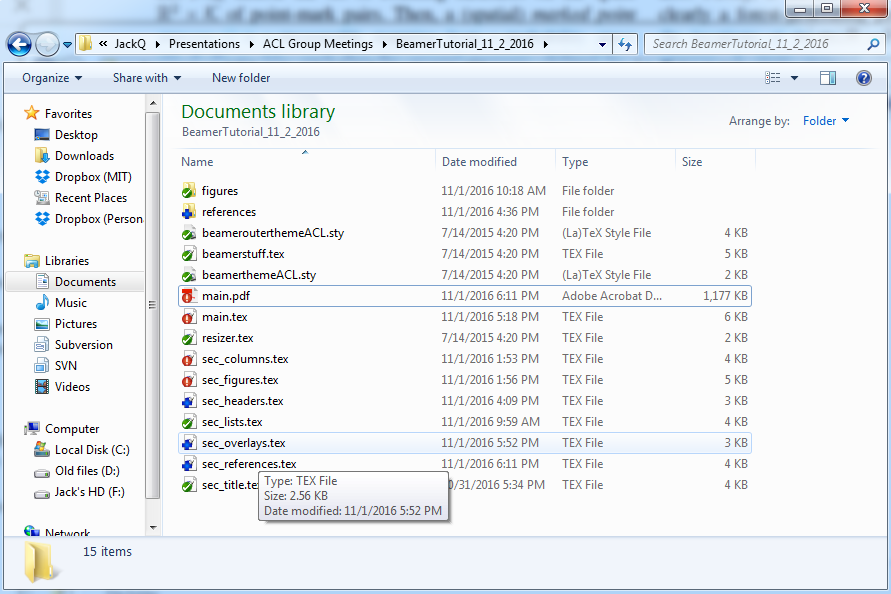
\includegraphics[width=0.95\columnwidth]{figures/folderView.png}
	\end{center}
\end{frame}


\end{document} %Need this to end the document
